\documentclass[12pt,a4paper]{report}

% ------------------------------------------------------------
% Rapport de projet - MeloStream
% ------------------------------------------------------------

\usepackage[utf8]{inputenc}
\usepackage[T1]{fontenc}
\usepackage[french]{babel}
\usepackage{geometry}
\usepackage{graphicx}
\usepackage[table]{xcolor}
\usepackage{booktabs}
\usepackage{tabularx}
\usepackage{longtable}
\usepackage{array}
\usepackage{enumitem}
\usepackage{hyperref}
\usepackage{fancyhdr}
\usepackage{titlesec}
\usepackage{listings}
\usepackage{tikz}
\usepackage{float}
\usepackage{caption}

\usetikzlibrary{arrows.meta,positioning,shapes.geometric,fit}
\graphicspath{{images/}}

\geometry{top=2.3cm,bottom=2.3cm,left=2.5cm,right=2.5cm}
\setlength{\parindent}{0pt}
\setlength{\parskip}{0.45em}
\emergencystretch=2em

\definecolor{primary}{HTML}{0F766E}
\definecolor{secondary}{HTML}{2563EB}
\definecolor{dark}{HTML}{111827}
\definecolor{muted}{HTML}{6B7280}
\definecolor{light}{HTML}{F3F4F6}
\definecolor{line}{HTML}{D1D5DB}
\definecolor{codebg}{HTML}{F8FAFC}

\hypersetup{
    colorlinks=true,
    linkcolor=primary,
    urlcolor=secondary,
    citecolor=primary,
    pdftitle={Rapport de projet MeloStream},
    pdfauthor={Ayoub}
}

\pagestyle{fancy}
\fancyhf{}
\lhead{\textcolor{primary}{MeloStream}}
\rhead{Rapport de projet}
\cfoot{\thepage}
\renewcommand{\headrulewidth}{0.4pt}

\titleformat{\chapter}[display]
  {\normalfont\bfseries\color{dark}}
  {\Large\textcolor{primary}{Chapitre \thechapter}}
  {0.2cm}
  {\Huge}

\titleformat{\section}
  {\normalfont\Large\bfseries\color{primary}}
  {\thesection}
  {0.5em}
  {}

\titleformat{\subsection}
  {\normalfont\large\bfseries\color{dark}}
  {\thesubsection}
  {0.5em}
  {}

\setlist[itemize]{leftmargin=1.1cm,itemsep=0.15em}
\setlist[enumerate]{leftmargin=1.1cm,itemsep=0.15em}
\renewcommand{\arraystretch}{1.25}

\lstset{
    basicstyle=\ttfamily\small,
    backgroundcolor=\color{codebg},
    frame=single,
    rulecolor=\color{line},
    breaklines=true,
    columns=fullflexible,
    keepspaces=true
}

\newcommand{\projectName}{MeloStream}
\newcommand{\code}[1]{\texttt{#1}}
\newcommand{\tableHeader}{\rowcolor{primary!12}}

\begin{document}

% ------------------------------------------------------------
% Page de garde
% ------------------------------------------------------------

\begin{titlepage}
    \centering
    \vspace*{1.5cm}

    {\Huge\bfseries\textcolor{primary}{\projectName}\par}
    \vspace{0.3cm}
    {\Large Plateforme de streaming musical\par}

    \vspace{1.2cm}
    \begin{tikzpicture}
        \node[
            rounded corners=14pt,
            draw=primary,
            line width=1pt,
            fill=primary!7,
            minimum width=0.78\textwidth,
            minimum height=3.2cm,
            align=center
        ] {
            {\Large \textbf{Rapport de projet}}\\[0.25cm]
            Application web full-stack avec Spring Boot, Angular et MySQL
        };
    \end{tikzpicture}

    \vfill

    \begin{tabular}{rl}
        \textbf{Réalisé par :} & Ayoub \\
        \textbf{Type :} & Projet web full-stack \\
        \textbf{Backend :} & Java 21, Spring Boot \\
        \textbf{Frontend :} & Angular, TypeScript \\
        \textbf{Base de données :} & MySQL \\
        \textbf{Année universitaire :} & 2025--2027 \\
    \end{tabular}

    \vfill
    {\large \today\par}
\end{titlepage}

\tableofcontents
\newpage

% ------------------------------------------------------------
% Introduction
% ------------------------------------------------------------

\chapter*{Introduction}
\addcontentsline{toc}{chapter}{Introduction}

\section*{Contexte}
\addcontentsline{toc}{section}{Contexte}

Les plateformes musicales occupent aujourd'hui une place importante dans les
usages numériques. Elles permettent de rechercher des chansons, découvrir des
artistes, organiser ses préférences et partager facilement des titres avec
d'autres utilisateurs.

Le projet \projectName{} consiste à développer une application web de streaming
musical dans un contexte pédagogique. L'application propose une interface
moderne côté client, une API REST sécurisée côté serveur et une base de données
permettant de conserver les utilisateurs, les sessions et les titres favoris.

Le système utilise des services musicaux externes pour récupérer les chansons,
les artistes, les albums, les pochettes et les liens audio. Deezer est utilisé
par défaut pour les extraits audio, tandis que Jamendo peut être activé afin de
proposer des titres libres ou licenciés.

\section*{Objectifs}
\addcontentsline{toc}{section}{Objectifs}

Les objectifs du projet sont :

\begin{itemize}
    \item créer une application web complète avec une séparation claire entre
    frontend et backend ;
    \item permettre l'inscription, la connexion, la déconnexion et la gestion
    du profil utilisateur ;
    \item proposer un catalogue musical consultable par recherche ou par
    humeur ;
    \item intégrer un lecteur audio sans lancer automatiquement la musique après
    la connexion ;
    \item permettre la sauvegarde des titres favoris ;
    \item permettre la création de playlists et l'organisation des titres ;
    \item ajouter une fonctionnalité de partage de titre par lien ;
    \item fournir une interface d'administration protégée par rôle ;
    \item produire une documentation claire pour comprendre, lancer et maintenir
    le projet.
\end{itemize}

% ------------------------------------------------------------
% Cahier des charges
% ------------------------------------------------------------

\chapter{Cahier des charges}

\section{Problématique}

La problématique principale est de concevoir une plateforme musicale simple,
ergonomique et sécurisée, capable de relier une interface Angular à une API
Spring Boot et à une base de données MySQL. Le projet doit aussi communiquer
avec des API musicales externes sans rendre le code difficile à maintenir.

L'application doit donc répondre à trois exigences majeures :

\begin{itemize}
    \item fournir une expérience utilisateur fluide ;
    \item protéger les fonctionnalités privées par authentification ;
    \item garder une architecture technique claire et évolutive.
\end{itemize}

\section{Besoins identifiés}

\subsection{Besoins fonctionnels}

\begin{longtable}{|p{2.4cm}|p{11.2cm}|}
\hline
\tableHeader \textbf{Référence} & \textbf{Description} \\
\hline
BF01 & Créer un compte utilisateur. \\
\hline
BF02 & Se connecter et se déconnecter. \\
\hline
BF03 & Consulter et modifier son profil. \\
\hline
BF04 & Rechercher des titres par mot-clé, artiste, album ou humeur. \\
\hline
BF05 & Écouter un titre depuis un lecteur intégré. \\
\hline
BF06 & Ajouter un titre aux favoris. \\
\hline
BF07 & Supprimer un titre des favoris. \\
\hline
BF08 & Créer, renommer et supprimer une playlist. \\
\hline
BF09 & Ajouter ou retirer des titres d'une playlist. \\
\hline
BF10 & Partager un titre avec un lien direct. \\
\hline
BF11 & Charger automatiquement le titre ciblé lorsqu'un lien partagé est ouvert. \\
\hline
BF12 & Accéder à un espace administrateur pour gérer les utilisateurs. \\
\hline
\end{longtable}

\subsection{Besoins non fonctionnels}

\begin{longtable}{|p{2.4cm}|p{11.2cm}|}
\hline
\tableHeader \textbf{Référence} & \textbf{Description} \\
\hline
BNF01 & L'interface doit être responsive et lisible. \\
\hline
BNF02 & Les mots de passe doivent être stockés sous forme de hash. \\
\hline
BNF03 & Les endpoints privés doivent être protégés par jeton. \\
\hline
BNF04 & Les rôles doivent limiter l'accès à l'administration. \\
\hline
BNF05 & Le code doit être organisé par domaine fonctionnel. \\
\hline
BNF06 & La base de données doit être initialisée automatiquement en local. \\
\hline
BNF07 & Le projet doit être testable et documenté. \\
\hline
\end{longtable}

\section{Solutions proposées}

La solution proposée repose sur :

\begin{itemize}
    \item une application Angular pour l'interface utilisateur ;
    \item une API Spring Boot pour la logique métier et la sécurité ;
    \item une base MySQL pour la persistance ;
    \item une intégration Deezer/Jamendo pour les données musicales ;
    \item une authentification stateless par jeton ;
    \item une interface administrateur accessible seulement au rôle
    \code{ADMIN}.
\end{itemize}

% ------------------------------------------------------------
% Conception fonctionnelle
% ------------------------------------------------------------

\chapter{Conception fonctionnelle}

\section{Acteurs}

\begin{longtable}{|p{3.5cm}|p{10.1cm}|}
\hline
\tableHeader \textbf{Acteur} & \textbf{Rôle dans le système} \\
\hline
Visiteur & Peut créer un compte ou se connecter. \\
\hline
Utilisateur & Peut rechercher, écouter, sauvegarder, organiser et partager des titres. \\
\hline
Administrateur & Peut gérer les utilisateurs et consulter les statistiques. \\
\hline
API musicale externe & Fournit les titres, artistes, albums, images et audios. \\
\hline
\end{longtable}

\section{Diagramme de cas d'utilisation}

\begin{figure}[H]
\centering
\begin{tikzpicture}[
    actor/.style={draw, rounded corners, fill=secondary!10, minimum width=3.2cm, minimum height=0.8cm},
    usecase/.style={draw, ellipse, fill=primary!8, minimum width=3.8cm, minimum height=0.9cm, align=center},
    link/.style={-Latex, thick, color=muted}
]
    \node[actor] (visitor) {Visiteur};
    \node[actor, below=1.1cm of visitor] (user) {Utilisateur};
    \node[actor, below=1.1cm of user] (admin) {Administrateur};

    \node[usecase, right=3.2cm of visitor] (register) {S'inscrire};
    \node[usecase, below=0.6cm of register] (login) {Se connecter};
    \node[usecase, below=0.6cm of login] (search) {Rechercher};
    \node[usecase, below=0.6cm of search] (listen) {Écouter};
    \node[usecase, below=0.6cm of listen] (fav) {Gérer favoris};
    \node[usecase, below=0.6cm of fav] (playlist) {Gérer playlists};
    \node[usecase, below=0.6cm of playlist] (share) {Partager titre};
    \node[usecase, below=0.6cm of share] (manage) {Gérer utilisateurs};

    \draw[link] (visitor) -- (register);
    \draw[link] (visitor) -- (login);
    \draw[link] (user) -- (search);
    \draw[link] (user) -- (listen);
    \draw[link] (user) -- (fav);
    \draw[link] (user) -- (playlist);
    \draw[link] (user) -- (share);
    \draw[link] (admin) -- (manage);
\end{tikzpicture}
\caption{Diagramme de cas d'utilisation simplifié}
\end{figure}

\section{Diagramme de classes}

\begin{figure}[H]
\centering
\begin{tikzpicture}[
    class/.style={draw, rounded corners, fill=light, minimum width=4.2cm, align=left},
    relation/.style={-Latex, thick, color=muted}
]
    \node[class] (user) {
        \textbf{UserAccount}\\
        \rule{3.8cm}{0.2pt}\\
        id\\
        username\\
        email\\
        displayName\\
        passwordHash\\
        role
    };

    \node[class, right=2cm of user] (token) {
        \textbf{AuthToken}\\
        \rule{3.8cm}{0.2pt}\\
        id\\
        token\\
        user\\
        createdAt\\
        expiresAt
    };

    \node[class, below=1.4cm of user] (favorite) {
        \textbf{FavoriteTrack}\\
        \rule{3.8cm}{0.2pt}\\
        id\\
        user\\
        trackId\\
        title\\
        artist\\
        shareUrl
    };

    \node[class, right=2cm of favorite] (track) {
        \textbf{TrackDto}\\
        \rule{3.8cm}{0.2pt}\\
        id\\
        source\\
        title\\
        artist\\
        audioUrl\\
        tags
    };

    \draw[relation] (user) -- node[above]{1..*} (token);
    \draw[relation] (user) -- node[left]{1..*} (favorite);
    \draw[relation, dashed] (favorite) -- node[above]{référence} (track);
\end{tikzpicture}
\caption{Diagramme de classes principal}
\end{figure}

Le modèle est complété par les classes \code{Playlist} et
\code{PlaylistTrack}. Une playlist appartient à un utilisateur, et une playlist
contient plusieurs titres. Cette relation permet d'organiser les chansons au
delà de la simple liste de favoris.

\section{Scénario de partage d'un titre}

Le partage est une fonctionnalité importante de l'application. Elle permet à un
utilisateur de copier un lien vers un titre et à un autre utilisateur d'accéder
directement au même titre.

\begin{enumerate}
    \item L'utilisateur clique sur le bouton \textbf{Partager}.
    \item Le frontend construit une URL au format \code{?song=source:id}.
    \item Exemple : \url{http://localhost:4200/?song=deezer:3135556}.
    \item Un autre utilisateur ouvre ce lien.
    \item Après connexion, le frontend appelle l'API
    \path{/api/tracks/{source}/{trackId}}.
    \item Le titre est chargé dans la zone de lecture rapide.
    \item La musique ne démarre pas automatiquement.
\end{enumerate}

% ------------------------------------------------------------
% Conception technique
% ------------------------------------------------------------

\chapter{Conception technique}

\section{Architecture globale}

\begin{figure}[H]
\centering
\begin{tikzpicture}[
    box/.style={draw, rounded corners, fill=light, minimum width=4cm, minimum height=1cm, align=center},
    arrow/.style={-Latex, thick, color=primary}
]
    \node[box] (browser) {Navigateur\\Utilisateur};
    \node[box, below=1cm of browser] (angular) {Frontend Angular\\TypeScript + CSS};
    \node[box, below=1cm of angular] (spring) {Backend Spring Boot\\API REST sécurisée};
    \node[box, below left=1cm and 0.4cm of spring] (mysql) {MySQL\\users, tokens, favoris, playlists};
    \node[box, below right=1cm and 0.4cm of spring] (music) {APIs musicales\\Deezer / Jamendo};

    \draw[arrow] (browser) -- (angular);
    \draw[arrow] (angular) -- node[right]{/api} (spring);
    \draw[arrow] (spring) -- node[left]{JPA} (mysql);
    \draw[arrow] (spring) -- node[right]{RestClient} (music);
\end{tikzpicture}
\caption{Architecture technique de MeloStream}
\end{figure}

\section{Technologies utilisées}

\begin{longtable}{|p{3.6cm}|p{10cm}|}
\hline
\tableHeader \textbf{Couche} & \textbf{Technologies} \\
\hline
Frontend & Angular 21, TypeScript, RxJS, CSS responsive, \code{@lucide/angular}. \\
\hline
Backend & Java 21, Spring Boot 4.0.6, Spring Web MVC, Spring Security, Spring Data JPA. \\
\hline
Base de données & MySQL avec accès possible via phpMyAdmin. \\
\hline
APIs externes & Deezer public API et Jamendo API optionnelle. \\
\hline
Tests & Spring Boot Test, H2 pour les tests backend, Angular/Vitest côté frontend. \\
\hline
\end{longtable}

\section{Structure du projet}

\begin{lstlisting}
project web/
  backend/
    src/main/java/com/musicstream/
      admin/
      auth/
      config/
      deezer/
      favorites/
      jamendo/
      music/
      security/
    src/main/resources/application.yml
    pom.xml
  frontend/
    src/app/
      admin-api.ts
      app.css
      app.html
      app.spec.ts
      app.ts
      auth-api.ts
      favorite-api.ts
      music-api.ts
    package.json
    proxy.conf.json
  rapport/
    rapport.tex
    rapport.pdf
  README.md
\end{lstlisting}

\section{Sécurité}

La sécurité est assurée par Spring Security. L'application utilise un modèle
stateless : après connexion, le backend génère un jeton stocké en base dans la
table \code{auth\_tokens}. Le frontend transmet ensuite ce jeton pour accéder
aux endpoints protégés.

\begin{itemize}
    \item \path{/api/auth/login} et \path{/api/auth/register} sont publics.
    \item Les endpoints \path{/api/**} nécessitent une authentification.
    \item Les endpoints \path{/api/admin/**} nécessitent le rôle \code{ADMIN}.
    \item Les mots de passe sont hashés avant stockage.
    \item Les règles CORS autorisent le frontend local sur le port 4200.
\end{itemize}

\section{Endpoints REST principaux}

\begin{longtable}{|p{2.3cm}|p{5.6cm}|p{5.7cm}|}
\hline
\tableHeader \textbf{Méthode} & \textbf{Endpoint} & \textbf{Description} \\
\hline
\code{POST} & \path{/api/auth/register} & Créer un compte. \\
\hline
\code{POST} & \path{/api/auth/login} & Se connecter. \\
\hline
\code{GET} & \path{/api/auth/me} & Récupérer l'utilisateur connecté. \\
\hline
\code{PUT} & \path{/api/auth/profile} & Modifier le profil. \\
\hline
\code{POST} & \path{/api/auth/logout} & Se déconnecter. \\
\hline
\code{GET} & \path{/api/tracks} & Rechercher des titres. \\
\hline
\code{GET} & \path{/api/tracks/{source}/{trackId}} & Charger un titre partagé. \\
\hline
\code{GET} & \path{/api/favorites} & Lister les favoris. \\
\hline
\code{POST} & \path{/api/favorites} & Ajouter un favori. \\
\hline
\code{DELETE} & \path{/api/favorites/{trackId}} & Supprimer un favori. \\
\hline
\code{GET} & \path{/api/playlists} & Lister les playlists. \\
\hline
\code{POST} & \path{/api/playlists} & Créer une playlist. \\
\hline
\code{PUT} & \path{/api/playlists/{playlistId}} & Renommer une playlist. \\
\hline
\code{DELETE} & \path{/api/playlists/{playlistId}} & Supprimer une playlist. \\
\hline
\code{POST} & \path{/api/playlists/{playlistId}/tracks} & Ajouter un titre à une playlist. \\
\hline
\code{DELETE} & \path{/api/playlists/{playlistId}/tracks/{source}/{trackId}} & Retirer un titre d'une playlist. \\
\hline
\code{GET} & \path{/api/admin/stats} & Consulter les statistiques. \\
\hline
\code{GET} & \path{/api/admin/users} & Lister les utilisateurs. \\
\hline
\code{PUT} & \path{/api/admin/users/{userId}/role} & Modifier un rôle. \\
\hline
\code{DELETE} & \path{/api/admin/users/{userId}} & Supprimer un utilisateur. \\
\hline
\end{longtable}

% ------------------------------------------------------------
% Réalisation
% ------------------------------------------------------------

\chapter{Réalisation}

\section{Fonctionnalités développées}

\subsection{Authentification}

L'utilisateur peut créer un compte, se connecter et se déconnecter. Après une
connexion réussie, un jeton est utilisé pour sécuriser les requêtes suivantes.
Les comptes de démonstration sont créés automatiquement au démarrage.

\subsection{Recherche musicale}

Le catalogue permet de rechercher des titres par mot-clé. L'utilisateur peut
chercher un titre, un artiste ou un album. Le backend interroge les services
musicaux externes et retourne des objets normalisés au frontend.

\subsection{Lecture}

Chaque titre peut être lancé depuis l'interface. Une attention particulière a
été portée au comportement après connexion : l'application ne lance pas la
musique automatiquement.

\subsection{Favoris}

Un utilisateur connecté peut sauvegarder un titre dans ses favoris et le
retrouver plus tard. Les favoris sont persistés dans la base MySQL.

\subsection{Playlists}

L'utilisateur peut créer des playlists personnalisées, les renommer, les
supprimer et y ajouter des chansons depuis le catalogue ou la bibliothèque. Les
titres d'une playlist peuvent ensuite être écoutés, partagés ou retirés.

\subsection{Partage}

Chaque chanson possède un bouton de partage. Le lien généré contient la source
et l'identifiant du titre. Exemple :

\begin{lstlisting}
http://localhost:4200/?song=deezer:3135556
\end{lstlisting}

Lorsqu'un autre utilisateur ouvre ce lien, le titre est chargé après
authentification.

\subsection{Administration}

Les comptes administrateurs peuvent consulter les statistiques, lister les
utilisateurs, modifier les rôles et supprimer un utilisateur autre que leur
propre compte.

\section{Captures d'écran}

Les captures suivantes ont été réalisées sur l'application locale. Elles
présentent les principaux écrans développés : authentification, inscription,
catalogue, recherche, partage, favoris, playlists, paramètres et administration.

\begin{figure}[H]
    \centering
    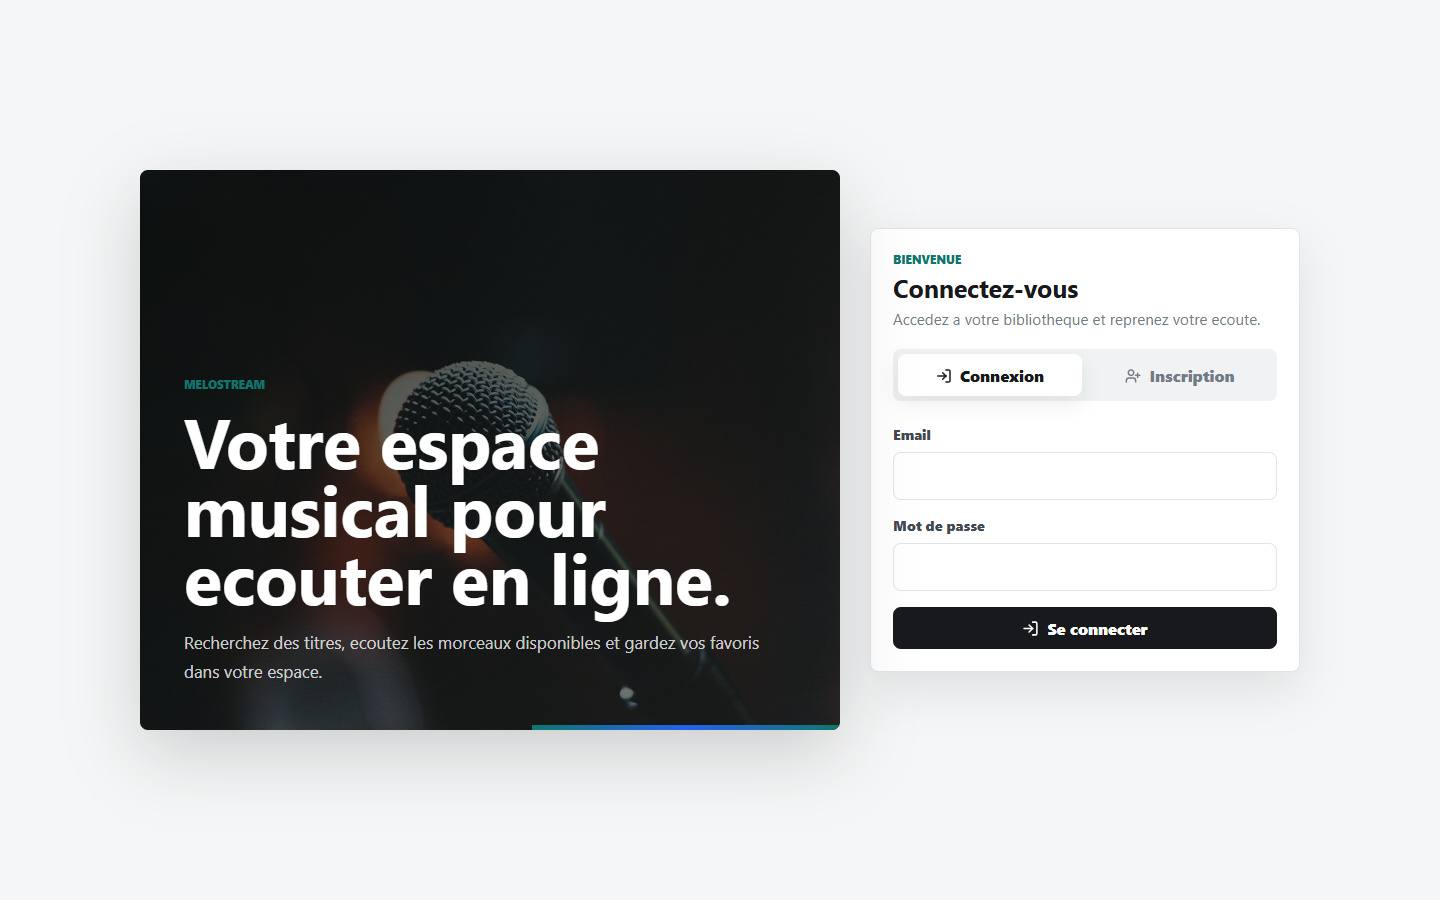
\includegraphics[width=\textwidth]{01-authentification.png}
    \caption{Page d'authentification}
\end{figure}

\begin{figure}[H]
    \centering
    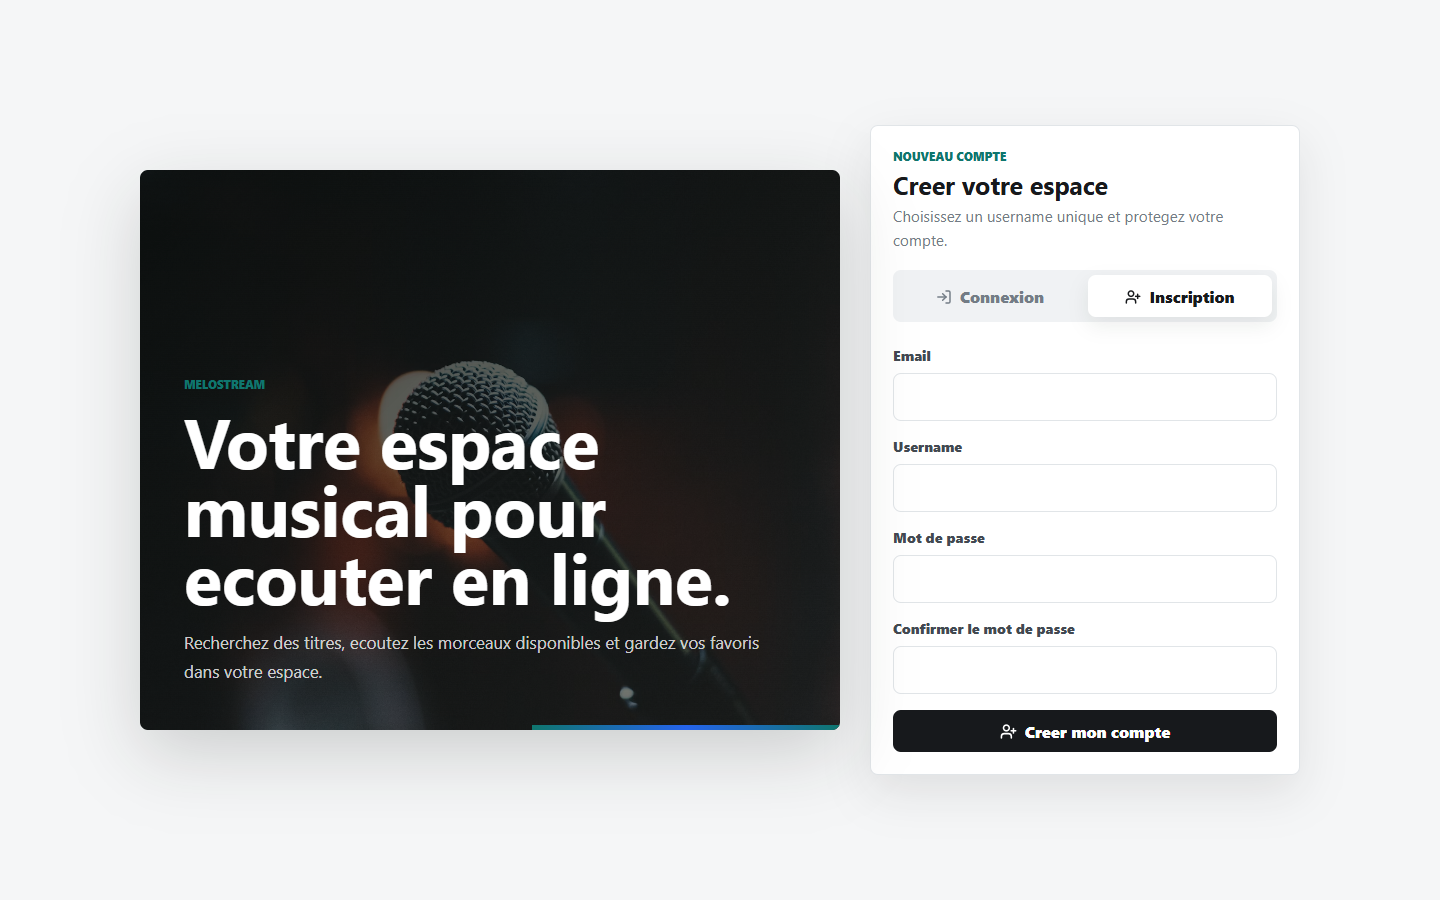
\includegraphics[width=\textwidth]{08-inscription-utilisateur.png}
    \caption{Page d'inscription utilisateur}
\end{figure}

\begin{figure}[H]
    \centering
    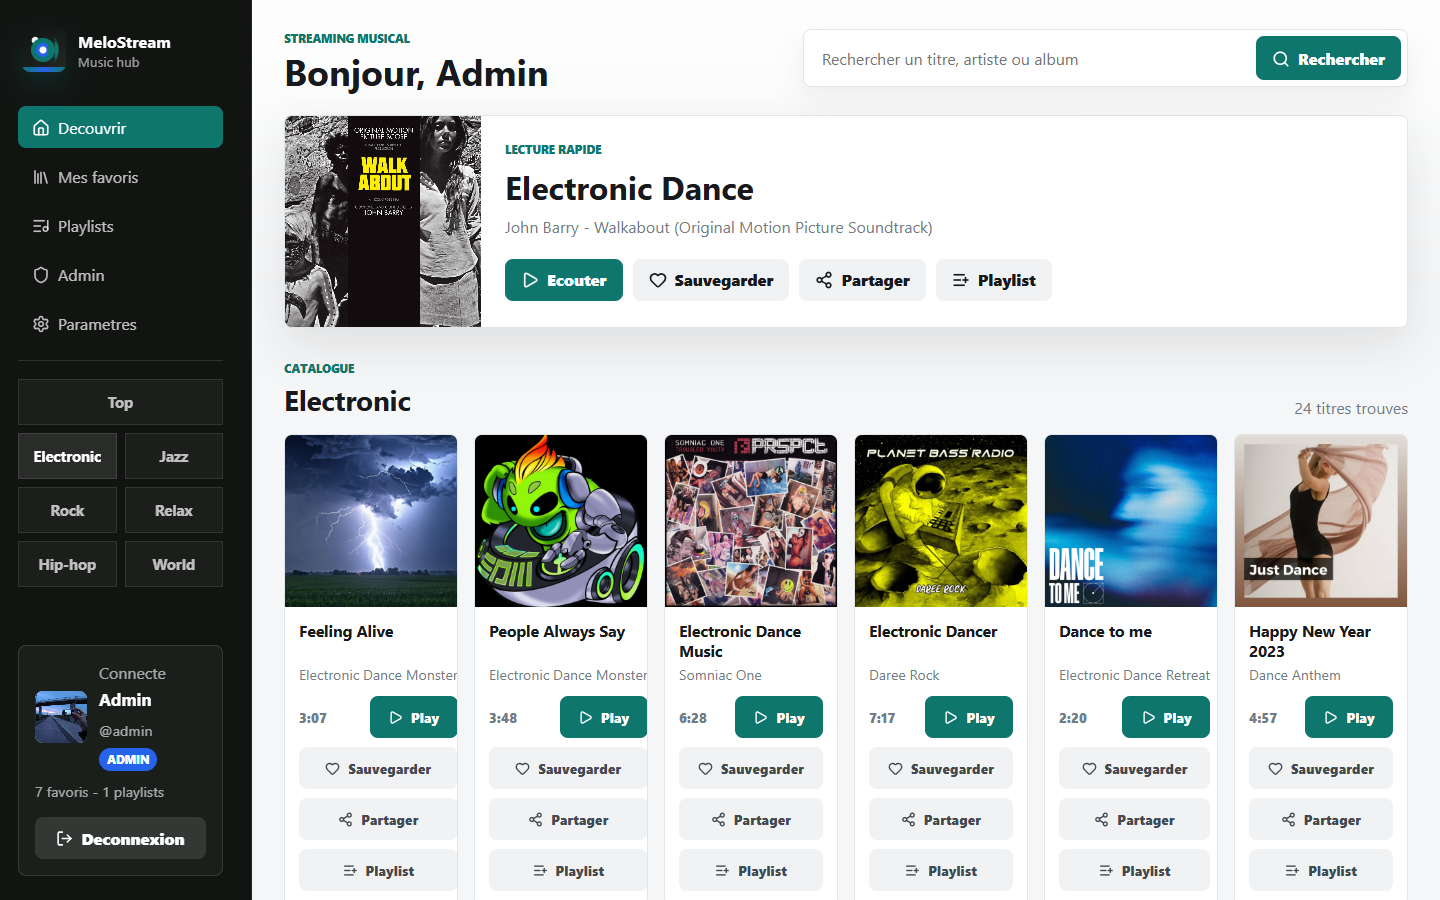
\includegraphics[width=\textwidth]{02-accueil-catalogue.png}
    \caption{Accueil utilisateur et catalogue musical}
\end{figure}

\begin{figure}[H]
    \centering
    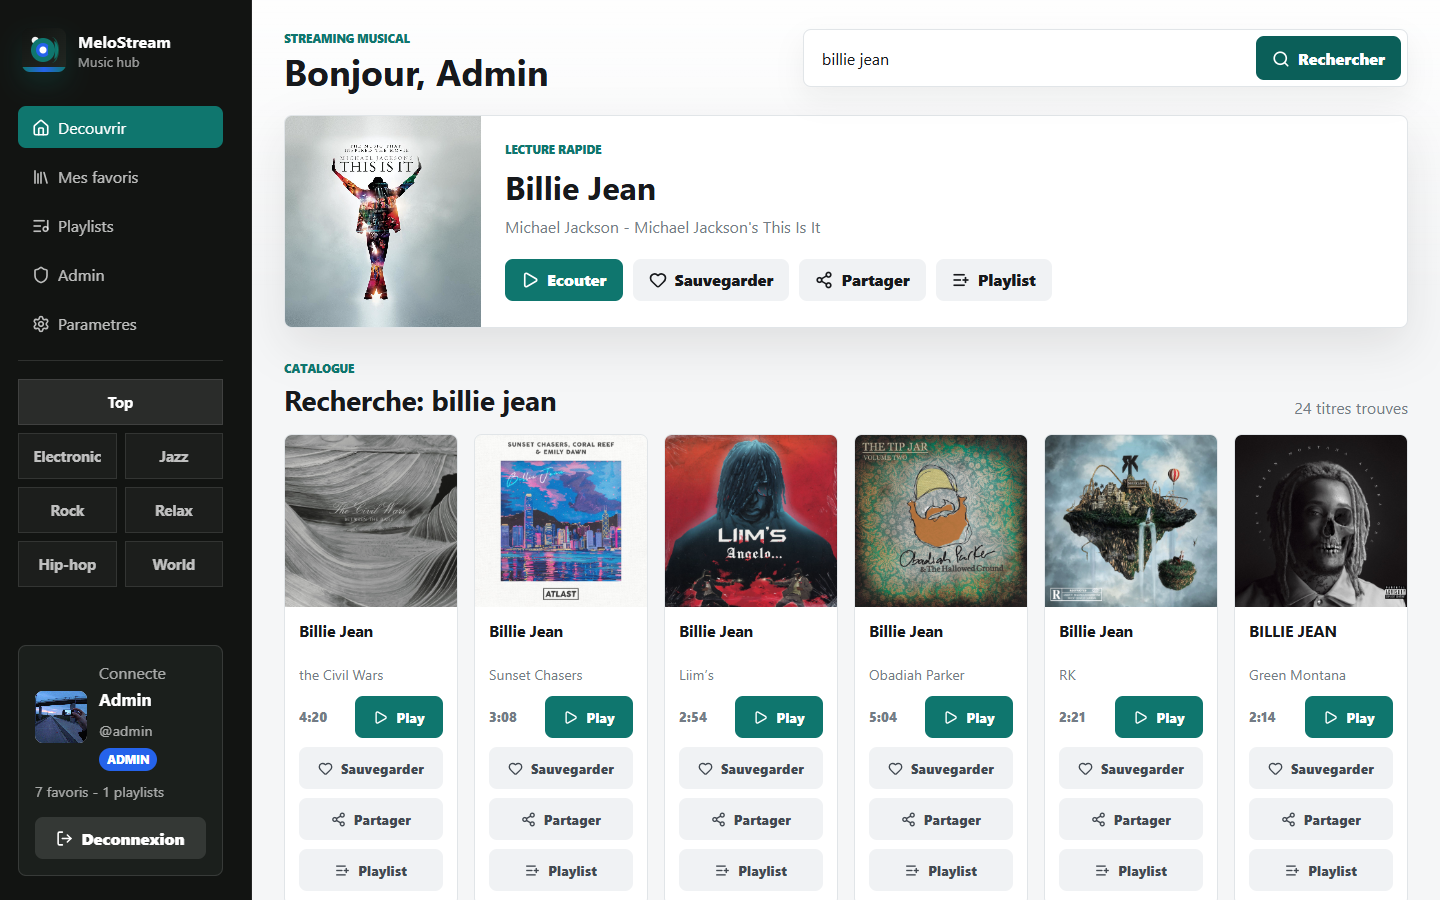
\includegraphics[width=\textwidth]{07-recherche-chanson.png}
    \caption{Résultats d'une recherche de chanson}
\end{figure}

\begin{figure}[H]
    \centering
    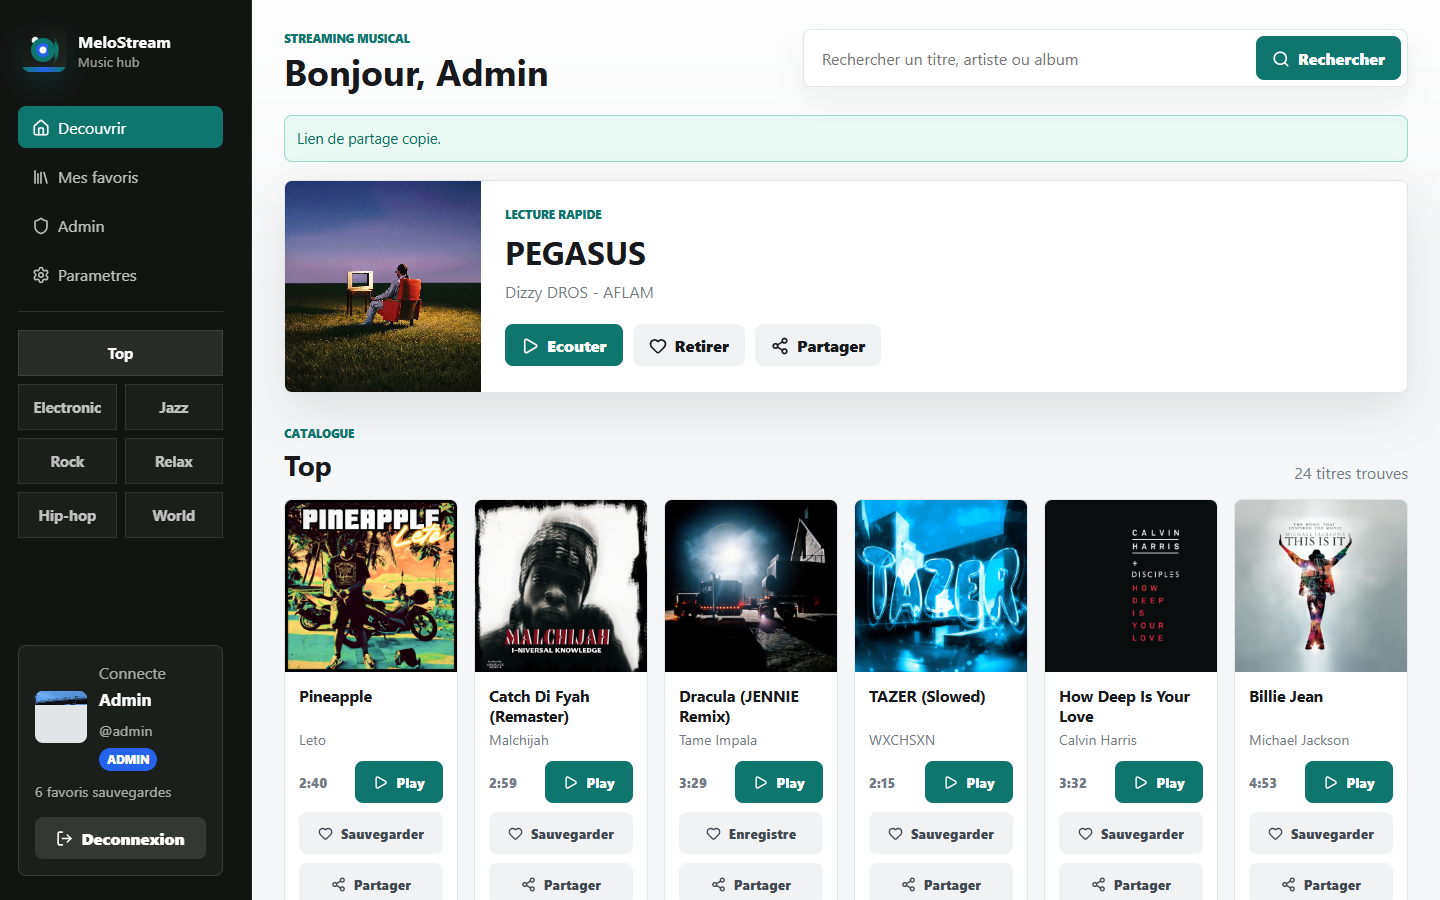
\includegraphics[width=\textwidth]{03-partage-titre.png}
    \caption{Message affiché après le partage d'un titre}
\end{figure}

\begin{figure}[H]
    \centering
    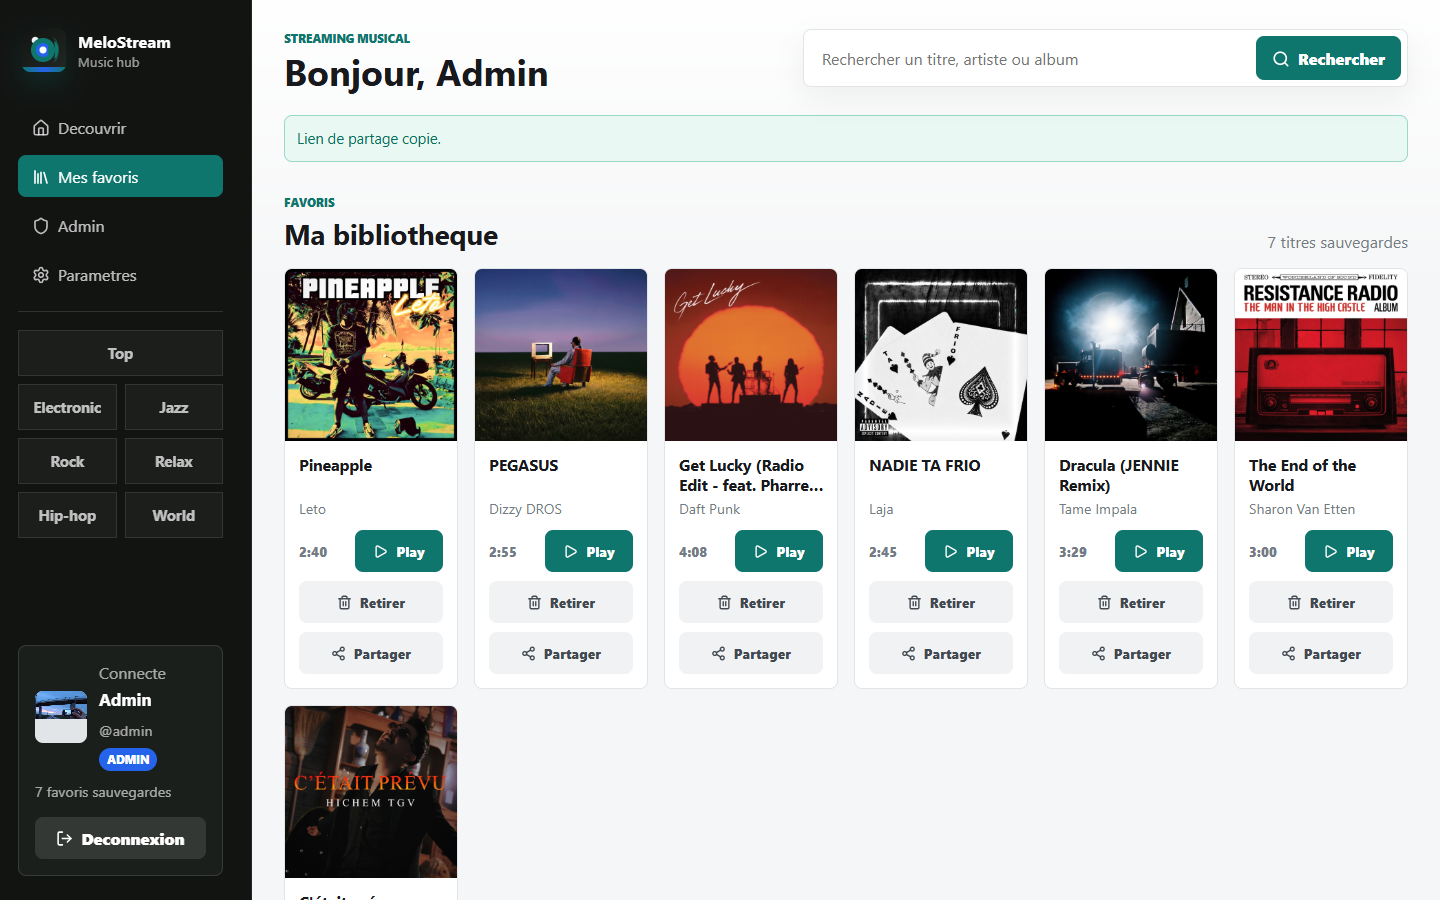
\includegraphics[width=\textwidth]{04-favoris.png}
    \caption{Bibliothèque des titres favoris}
\end{figure}

\begin{figure}[H]
    \centering
    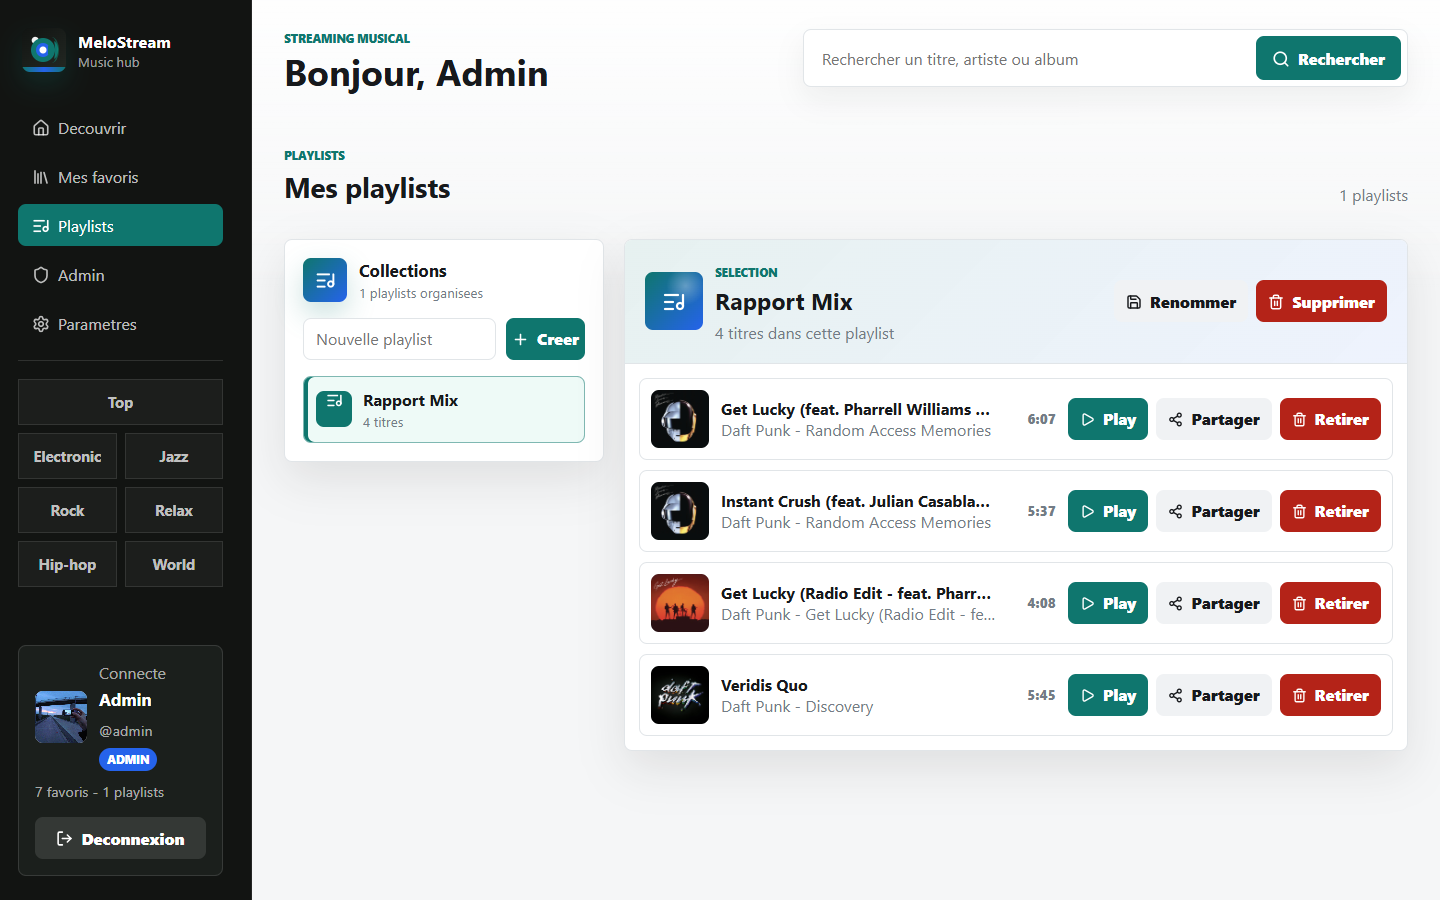
\includegraphics[width=\textwidth]{09-playlists.png}
    \caption{Gestion des playlists utilisateur}
\end{figure}

\begin{figure}[H]
    \centering
    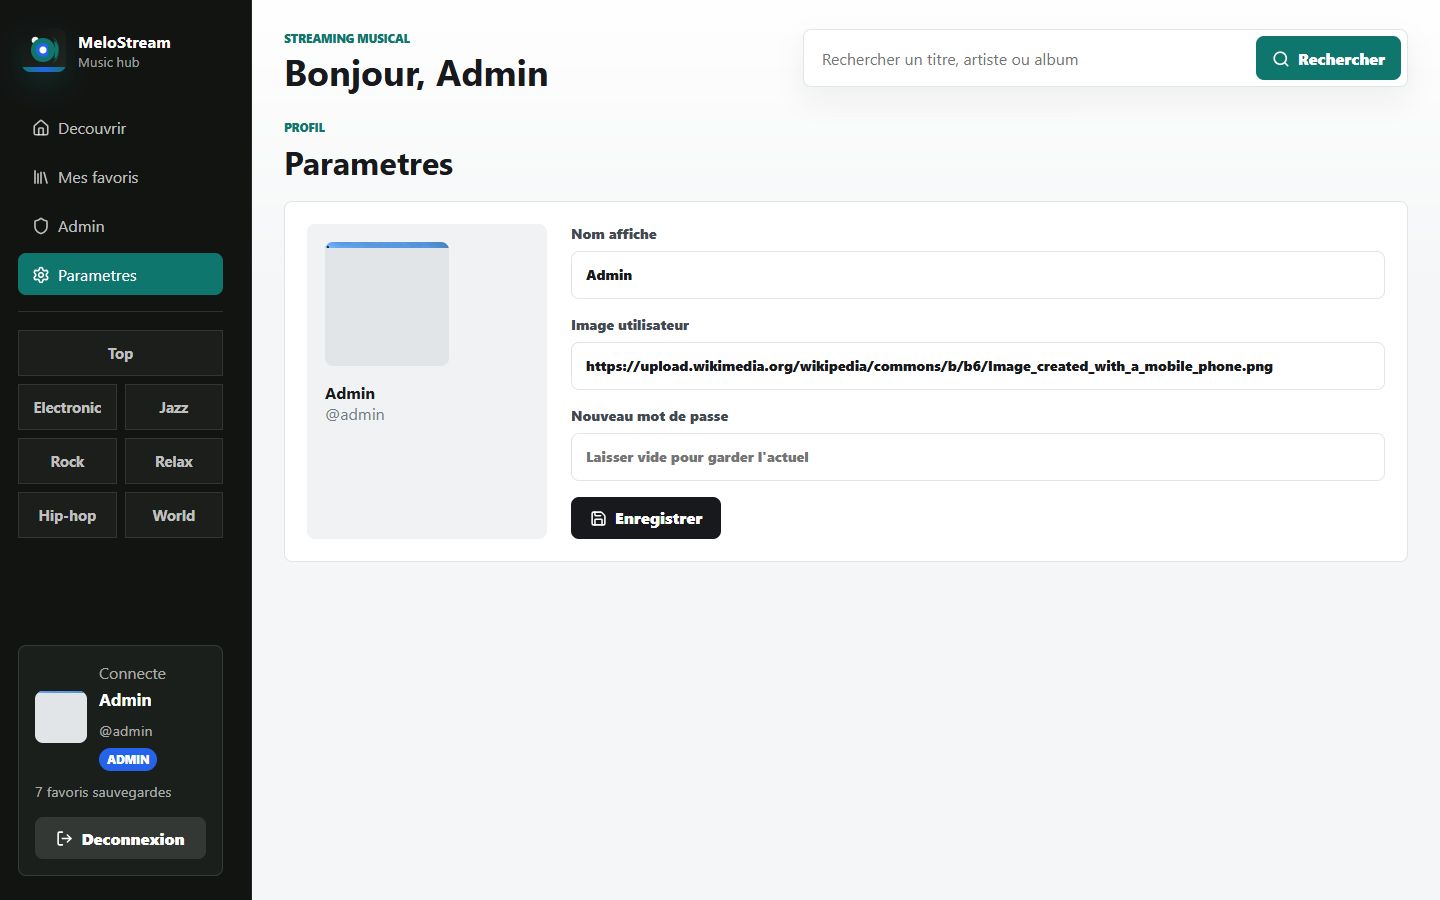
\includegraphics[width=\textwidth]{06-parametres.png}
    \caption{Page des paramètres du profil}
\end{figure}

\begin{figure}[H]
    \centering
    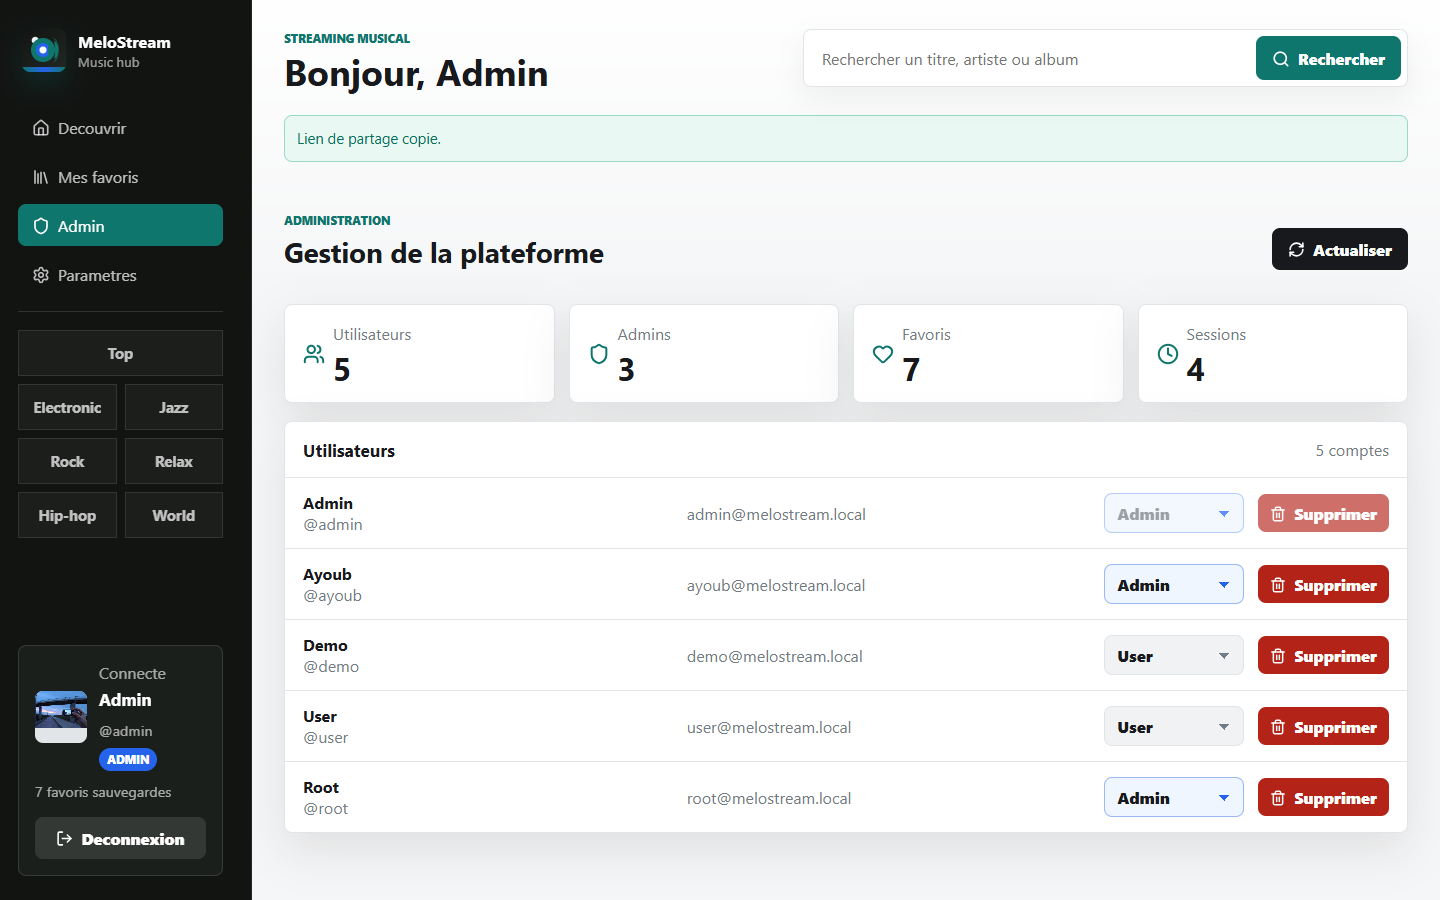
\includegraphics[width=\textwidth]{05-administration.png}
    \caption{Interface d'administration}
\end{figure}

\section{Comptes de démonstration}

\begin{longtable}{|p{6cm}|p{4cm}|p{3cm}|}
\hline
\tableHeader \textbf{Email} & \textbf{Mot de passe} & \textbf{Rôle} \\
\hline
\code{admin@melostream.local} & \code{admin123} & \code{ADMIN} \\
\hline
\code{ayoub@melostream.local} & \code{ayoub123} & \code{USER} \\
\hline
\code{demo@melostream.local} & \code{demo123} & \code{USER} \\
\hline
\code{user@melostream.local} & \code{user123} & \code{USER} \\
\hline
\code{root@melostream.local} & \code{root123} & \code{ADMIN} \\
\hline
\end{longtable}

% ------------------------------------------------------------
% Installation
% ------------------------------------------------------------

\chapter{Installation et lancement}

\section{Prérequis}

\begin{itemize}
    \item Java 21.
    \item Node.js et npm.
    \item MySQL local.
    \item Maven Wrapper inclus dans le backend.
\end{itemize}

\section{Configuration de la base}

La configuration par défaut utilise MySQL en local :

\begin{lstlisting}
database: music_stream
username: root
password: vide
\end{lstlisting}

La base est créée automatiquement grâce à l'option
\code{createDatabaseIfNotExist=true}.

\section{Lancement du backend}

\begin{lstlisting}
cd backend
.\mvnw.cmd spring-boot:run
\end{lstlisting}

Le backend démarre sur :

\begin{lstlisting}
http://localhost:8080
\end{lstlisting}

\section{Lancement du frontend}

\begin{lstlisting}
cd frontend
npm install
npm start
\end{lstlisting}

Le frontend démarre sur :

\begin{lstlisting}
http://localhost:4200
\end{lstlisting}

\section{Activation optionnelle de Jamendo}

Pour utiliser Jamendo, il faut définir la variable d'environnement suivante
avant de lancer le backend :

\begin{lstlisting}
$env:JAMENDO_CLIENT_ID="ton_client_id_jamendo"
\end{lstlisting}

% ------------------------------------------------------------
% Vérification
% ------------------------------------------------------------

\chapter{Vérification}

\section{Tests backend}

\begin{lstlisting}
cd backend
.\mvnw.cmd test
\end{lstlisting}

\section{Tests frontend}

\begin{lstlisting}
cd frontend
npm test -- --watch=false
\end{lstlisting}

\section{Build frontend}

\begin{lstlisting}
cd frontend
npm run build
\end{lstlisting}

% ------------------------------------------------------------
% Conclusion
% ------------------------------------------------------------

\chapter*{Conclusion}
\addcontentsline{toc}{chapter}{Conclusion}

Le projet \projectName{} répond aux objectifs fixés : il propose une plateforme
musicale complète avec authentification, recherche, lecture, favoris, playlists,
partage et administration. L'architecture sépare clairement le frontend Angular, le
backend Spring Boot et la base MySQL, ce qui facilite la maintenance et les
évolutions futures.

Les principaux défis rencontrés concernent l'intégration des API musicales
externes, la gestion des liens de partage et la sécurisation des endpoints. Le
projet peut encore être amélioré avec une route Angular dédiée au partage, une
documentation OpenAPI, davantage de tests d'intégration et une configuration de
déploiement adaptée à la production.

\end{document}
